\chapter{\textbf{Cloud infrastructure management}}
\label{chap:infrastructure}

This section will be used to describe OpenNebula, the virtual infrastructure (VI) manager chosen to have the virtualization design advisor implemented over. Organizations can use it to manage and deploy VMs, individually or in groups that must be co-scheduled on local or external resources. It merges a lot of different technologies, in order to allow users to design their private or hybrid clouds. Some of its key features are:
\begin{itemize}
 \item It provides a homogeneous view of resources, regardless of the underlying hypervisor (e.g. KVM, Xen, etc.). This makes the virtualization much less restrictive. The physical machine in which the VM is being run does not need to be tied to a specific virtualization technology, which may cause incompatibility issues;
  \item It manages a VM full life cycle, it is used to specify storage requirements and setting up the network;
  \item Supports configurable resource allocation policies.
\end{itemize}

The OpenNebula architecture is illustrated in figure ~\ref{fig:open_arch}. It can basically be split into three layers. The core (middle layer ), which has three management areas. One of them is dealing with the creation of virtual networks, which is done through the Virtual Network (VN) manager. This component is responsible for handing out and keeping track of leases ( composed by one IP and one MAC address valid on a particular network ), and their associations with VMs and physical bridges used. Second, it needs to manage and monitor the physical hosts, which is the responsibility of the host manager. And finally, there is the VM manager, responsible for taking care of a VM's life cycle. It prepares the disk images for them, by controlling the image and storage technologies. It also needs to control the hypervisors, responsible for their creation and control. And combined with the VN manager, this manager provides the VM with the network environment. Another important feature in the core is achieved with 
the SQL Pool. It is responsible for saving the OpenNebula state. Even after a shutdown or a failure, it is possible to restore a previous state. All the managers make use of this Pool to store information.


\begin{figure}[ht]
  \centering
 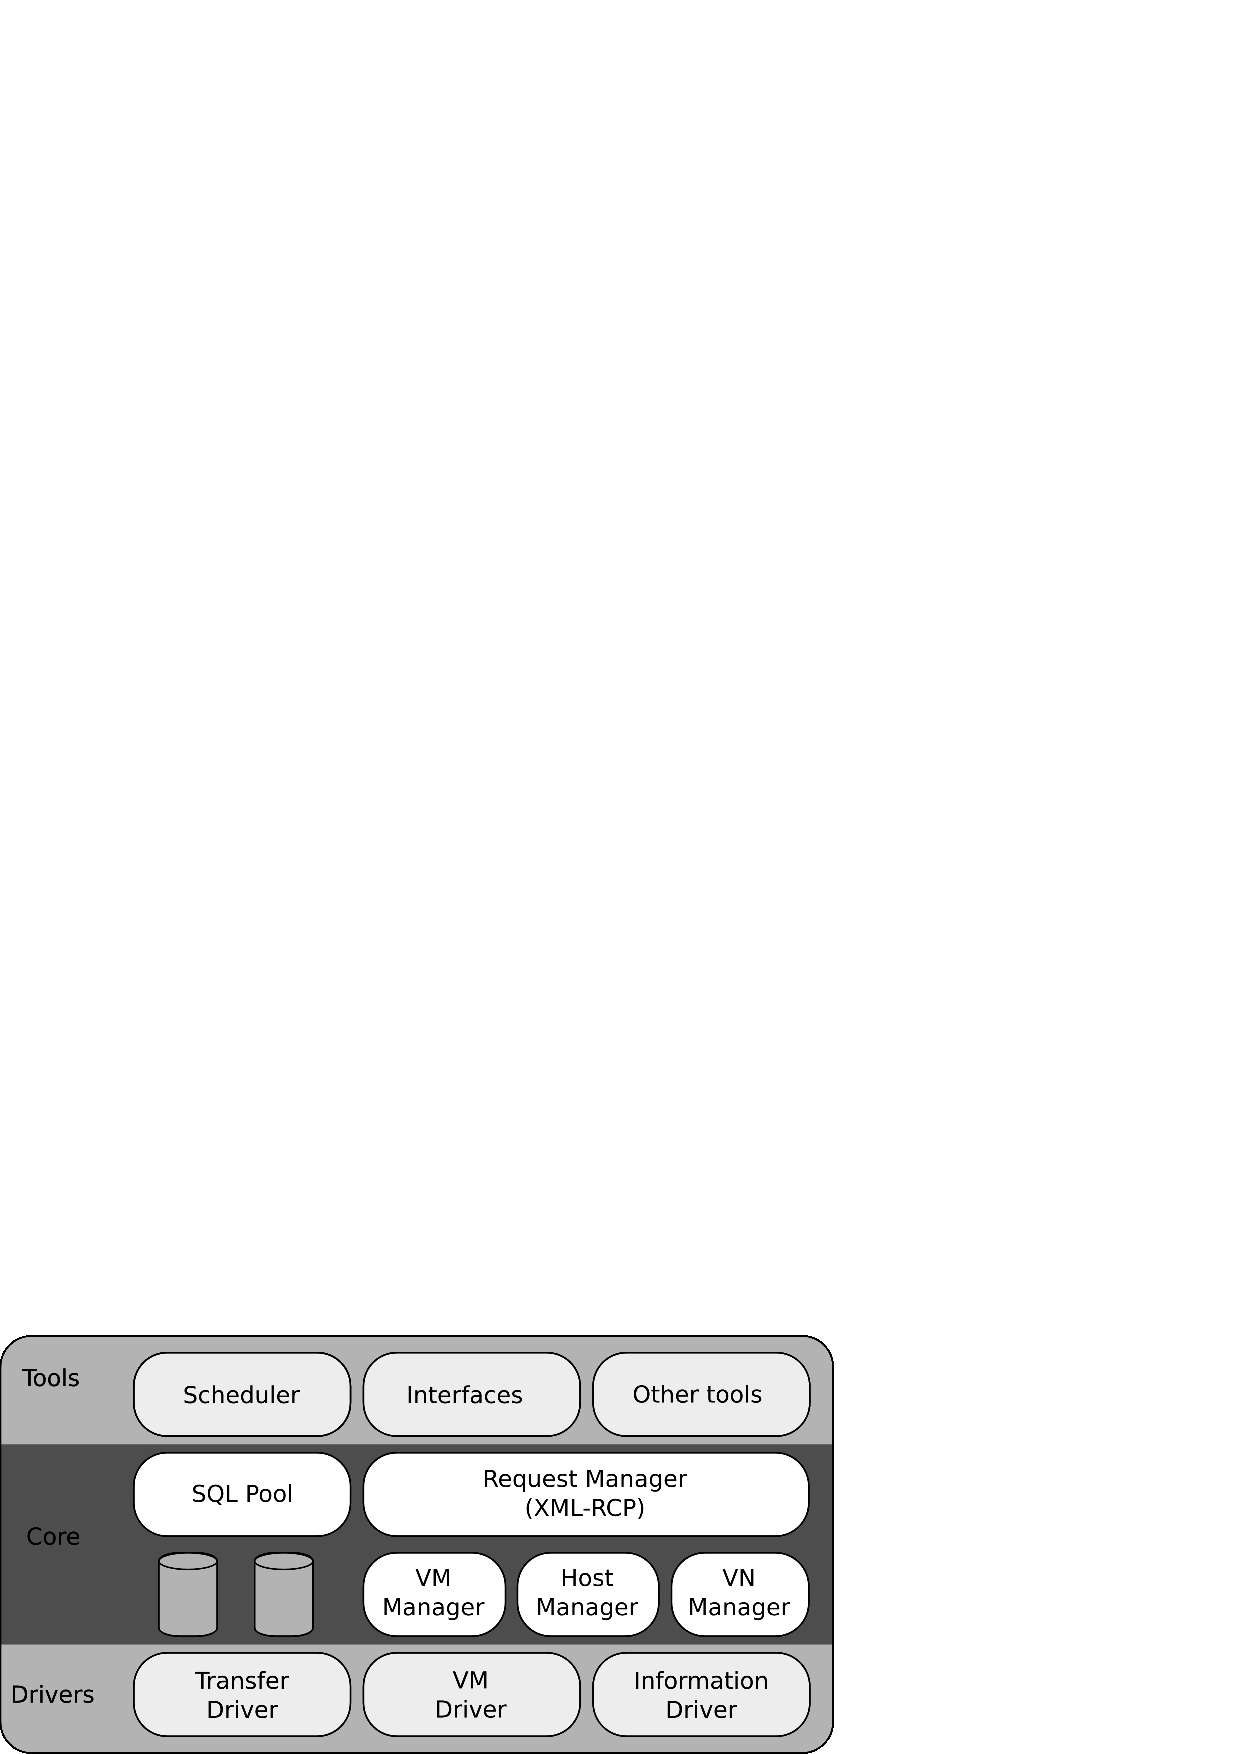
\includegraphics[scale=1]{one-architecture_2.png}
  \caption{OpenNebula architecture}
  \label{fig:open_arch}
\end{figure}

One important feature of the core module is the service deployment support. The Request manager exposes a XML-RPC interface that decouples most of the functionality present in the core. Through this interface it is possible to control and manage any OpenNebula resource, including virtual machines, networks, images, hosts, etc. As OpenNebula is in continuing development, it is expected that this API will support even more functionality. Currently, it is known that dynamic resource allocation is not supported yet. All the resource allocation is performed offline, through VM templates. The amount of resources allocated is passed from the templates directly to the hypervisors, and they will be the same until the end of that VM's life cycle. We will discuss more about this issue on the next chapter, as resource reallocation is important for the advisor.

All these described activities are performed through pluggable drivers, present in the bottom layer. This modularity makes the system easier to extend and avoids tying it to any specific technology. The drivers shown in figure ~\ref{fig:open_arch}  address some particular areas, such as virtualization ( by communicating with the hypervisor ), storage operations, gather monitoring information and authenticate user requests.

Other way of extending OpenNebula is through hooks, controlled by the Hook manager. They enable the triggering of custom scripts tied to a change in a particular resource, being that a Host or a Virtual Machine. This opens a wide area of automation for system administrators. Below is an example of a hook, namely "error", defined in the proper configuration file. It is used to perform recovery actions when a host fails ( i.e. it enters in the ERROR state ). When this happens, the script host\_error.rb is called with the host id passed as an argument. The "remote" parameter tells that this script should be executed in the OpenNebula server, and not in the failed host. The purpose of this script is to resubmit all the VMs that were running on the failed host, for them to be run on active hosts. 

\begin{itemize}
 \item HOST\_HOOK $=$ [ \\
    name      $=$ "error",\\
    on        $=$ "ERROR",\\
    command   $=$ "host\_error.rb",\\
    arguments $=$ "\$HID",\\
    remote    $=$ no ]\\
\end{itemize}

In the top layer there are user interfaces to access OpenNebula, and also APIs extended from the XML-RPC interface, which can work between the core and other tools. One of these APIs is  OCA\footnote{OpenNebula Cloud API}. It exposes the same functionality as XML-RPC, in a more convenient way. Other relevant module for this paper is the OpenNebula's scheduler, also in the top layer. Its job is to make placement decisions for the VMs ( i.e. it assigns physical machines for VMs ). It has access to all requests OpenNebula receives. Based on these requests, it keeps track on allocations and sends the appropriate deployment commands to OpenNebula's core. As other modules, it can be replaced by third party solutions, such as Haizea\footnote{http://haizea.cs.uchicago.edu/},  which offers more sophisticated placement policies. However, in this paper we will stick to the OpenNebula's default scheduler. Next, we will describe it in more details.

\section{Scheduler}

The scheduler already present in OpenNebula works only with immediate provisioning. Its concept is pretty straightforward, the resources are only provisioned at the moment they are required, if that is not possible, then the requirement is ignored. The requirements are done in a manual and static way, in which the amount of resources, among other configurations, are defined in a file. The assignment is performed through a classification policy.  The administrator needs to set a \textit{RANK} variable, which defines which host is more suitable for a VM. Each VM has its own \text{RANK} equation, and the scheduler assigns a host with the highest value for this variable to a VM. In OpenNebula, deployments are performed through VM templates, so you can share the same scheduling policy  to a group of VMs. For instance, here are some possible \textit{RANK} definitions, each one serving a specific policy:

\begin{itemize}
 \item Load-aware Policy
 \begin{itemize}
   \item \textbf{Heuristic:} Use nodes with less load;
   \item \textbf{Implementation:} Use nodes with more \textit{FREECPU} first.
    \item \textit{RANK} = \textit{FREECPU}

 \end{itemize}

  \item Striping policy
  \begin{itemize}
   \item \textbf{Heuristic:} Spread the VMs in the cluster node;
   \item \textbf{Implementation:} Use the nodes with less VMs running first.
   \item \textit{RANK} = "\textit{- RUNNING\_VMS}"
  \end{itemize}

\end{itemize}

Furthermore, users may use the same syntax applied to \textit{RANK} statements to define a \textit{REQUIREMENT}. Requirements are used to set placement constraints. They rule out hosts from the list of machines suitable to run a certain VM. Below is an example of a requirement statement. It only allows  a VM to be run by nodes with CPUs that have clock higher than $1000 MHz$:
\begin{itemize}
 \item \textit{REQUIREMENT} = \textit{CPUSPEED} $> 1000$ 
\end{itemize}


